\documentclass{standalone}
\usepackage[dvipsnames]{xcolor}
\usepackage{tikz}
\usetikzlibrary{calc}

\begin{document}

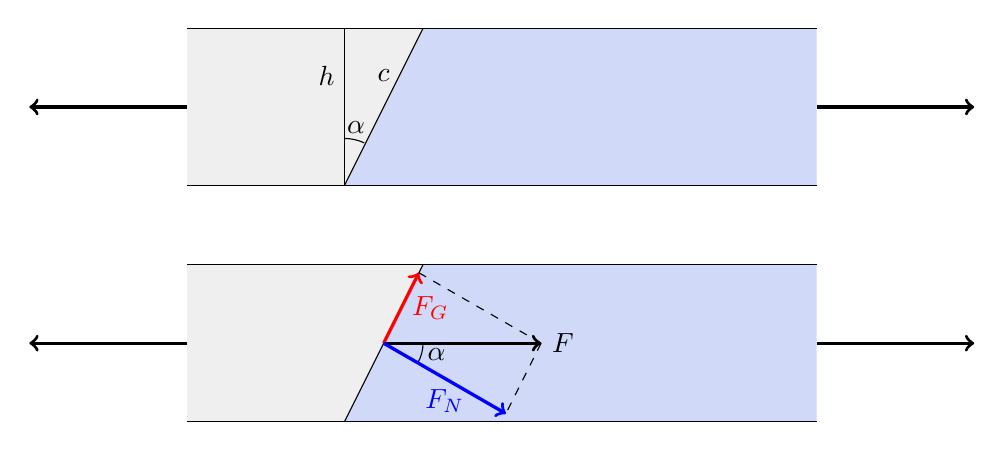
\begin{tikzpicture}[scale=2]
  \fill[lightgray!25!white] (0,0) -- (0.5,1) -- (-1,1) -- (-1,0);
  \fill[RoyalBlue!25!white] (0,0) -- (0.5,1) -- (3,1) -- (3,0);
  \draw (0,0.3) arc [start angle=90, end angle=65, radius = 0.3] node[above, xshift=-3pt]{$\alpha$};  
  % \draw (0.5,0.5) arc [start angle=0, end angle=-30, radius = 0.25] node[right, yshift=3pt]{$\alpha$};  
  \draw(-1,0) -- (3,0);
  \draw[->, very thick](-1,0.5) -- (-2,0.5);
  \draw[->, very thick](3,0.5) -- (4,0.5);
  \draw(-1,1) -- (3,1);
  \draw (0,0) -- node[left, pos=0.7]{$h$}(0,1);
  \draw (0,0) -- node[left, pos=0.7]{$c$}(0.5,1);
%   \begin{scope}[very thick]
% %  \draw[->] (0.25,0.5) -- (1.25,0.5);
%   \draw[->] (0.25,0.5) -- (1.25,0.5) node[right]{$F$}; 
%   \draw[->,red] (0.25,0.5) -- node[right]{$F_G$} (0.4736068, 0.9472136);
%   \draw[->,blue] (0.25,0.5) -- node[below]{$F_N$} ($(1.25,0.5)-(0.4736068, 0.9472136)+(0.25,0.5)$); 
%   \draw[dashed, thin](0.4736068, 0.9472136) --  (1.25,0.5);
%   \draw[dashed, thin](1.25, 0.5) --  ($(1.25,0.5)-(0.4736068, 0.9472136)+(0.25,0.5)$);
% \end{scope}
  \begin{scope}[yshift = -1.5cm]
  \fill[lightgray!25!white] (0,0) -- (0.5,1) -- (-1,1) -- (-1,0);
  \fill[RoyalBlue!25!white] (0,0) -- (0.5,1) -- (3,1) -- (3,0);
  % \draw (0,0.3) arc [start angle=90, end angle=60, radius = 0.3] node[above, xshift=-3pt]{$\alpha$};  
  \draw (0.5,0.5) arc [start angle=0, end angle=-30, radius = 0.25] node[right, yshift=3pt]{$\alpha$};  
  \draw(-1,0) -- (3,0);
  \draw[->, very thick](-1,0.5) -- (-2,0.5);
  \draw[->, very thick](3,0.5) -- (4,0.5);
  \draw(-1,1) -- (3,1);
  % \draw (0,0) -- node[left, pos=0.7]{$h$}(0,1);
  \draw (0,0) -- (0.5,1);
  \begin{scope}[very thick]
%  \draw[->] (0.25,0.5) -- (1.25,0.5);
  \draw[->] (0.25,0.5) -- (1.25,0.5) node[right]{$F$}; 
  \draw[->,red] (0.25,0.5) -- node[right]{$F_G$} (0.4736068, 0.9472136);
  \draw[->,blue] (0.25,0.5) -- node[below]{$F_N$} ($(1.25,0.5)-(0.4736068, 0.9472136)+(0.25,0.5)$); 
  \draw[dashed, thin](0.4736068, 0.9472136) --  (1.25,0.5);
  \draw[dashed, thin](1.25, 0.5) --  ($(1.25,0.5)-(0.4736068, 0.9472136)+(0.25,0.5)$);
\end{scope}
\end{scope}
\end{tikzpicture}


\end{document}
